\subsection{I beacon Bluetooth}
Per gestire la riproduzione automatizzata delle audioguide è stato deciso di usare dei beacon Bluetooth, dei piccoli dispositivi disponibili a un prezzo relativamente basso. 

\subsubsection{Cosa sono}
I \textbf{beacon Bluetooth} sono dei trasmettitori hardware - una classe di dispositivi \emph{Bluetooth low energy} che trasmettono il loro identificatore ai dispositivi elettronici portatili vicini. Questa tecnologia permette a smartphone, tablet e altri dispositivi di eseguire azioni quando sono in prossimità di essi. Il beacon, tuttavia, non è in grado di rilevare alcun segnale. Non richiede una connessione Internet e agisce come un emittente entro un raggio breve.\cite{what_are_beacons}


\subsubsection{Perché i beacon Bluetooth?}
Attraverso la precisa localizzazione (la distanza di trasmissione si aggira intorno ai 10-30 metri), i beacon creano un \textbf{engagement mirato}: nel contesto opportuno, al momento opportuno, al pubblico interessato. Per questo e per i \textbf{costi accessibili} (un dispositivo costa in media 10 euro) sono la scelta più adatta al caso d'uso desiderato.

\begin{center}
\begin{figure}[htp]
    \centering
    \includegraphics[width=10cm]{diagrams/diagramma_perchè_beacon.png}
    \caption{Comunicazione con Beacon}
    \label{fig:comunicazione_beacon}
\end{figure}
\end{center}

\subsubsection{In sintesi}
Riassumendo, la comunicazione sarà composta da due elementi:
\begin{itemize}
    \item \textbf{Dal presentatore}: il beacon bluetooth, questo spedisce soltanto informazioni. L’informazione standard dei beacon consiste in un \emph{UUID}, e solo un valore major o minor. Per
    % TODO: change UID 
    esempio: UUID: 9e747915-5996-4b5b-8d3f-335ba7d0745e Major ID: 1 Minor ID: 2. Il trasmettitore non fa niente altro che inviare questa informazione ogni frazione di secondo. Ogni \emph{UUID} sarà associato ad ogni stanza così il client sarà in grado di rilevare in che posizione l'utente si trova.
    \item \textbf{Dall'osservatore}: l'applicazione mobile, sarà responsabile di ricevere i segnali e di far partire o fermare l'audio in base alla posizione.
\end{itemize}

\begin{center}
\begin{figure}[htp]
    \centering
    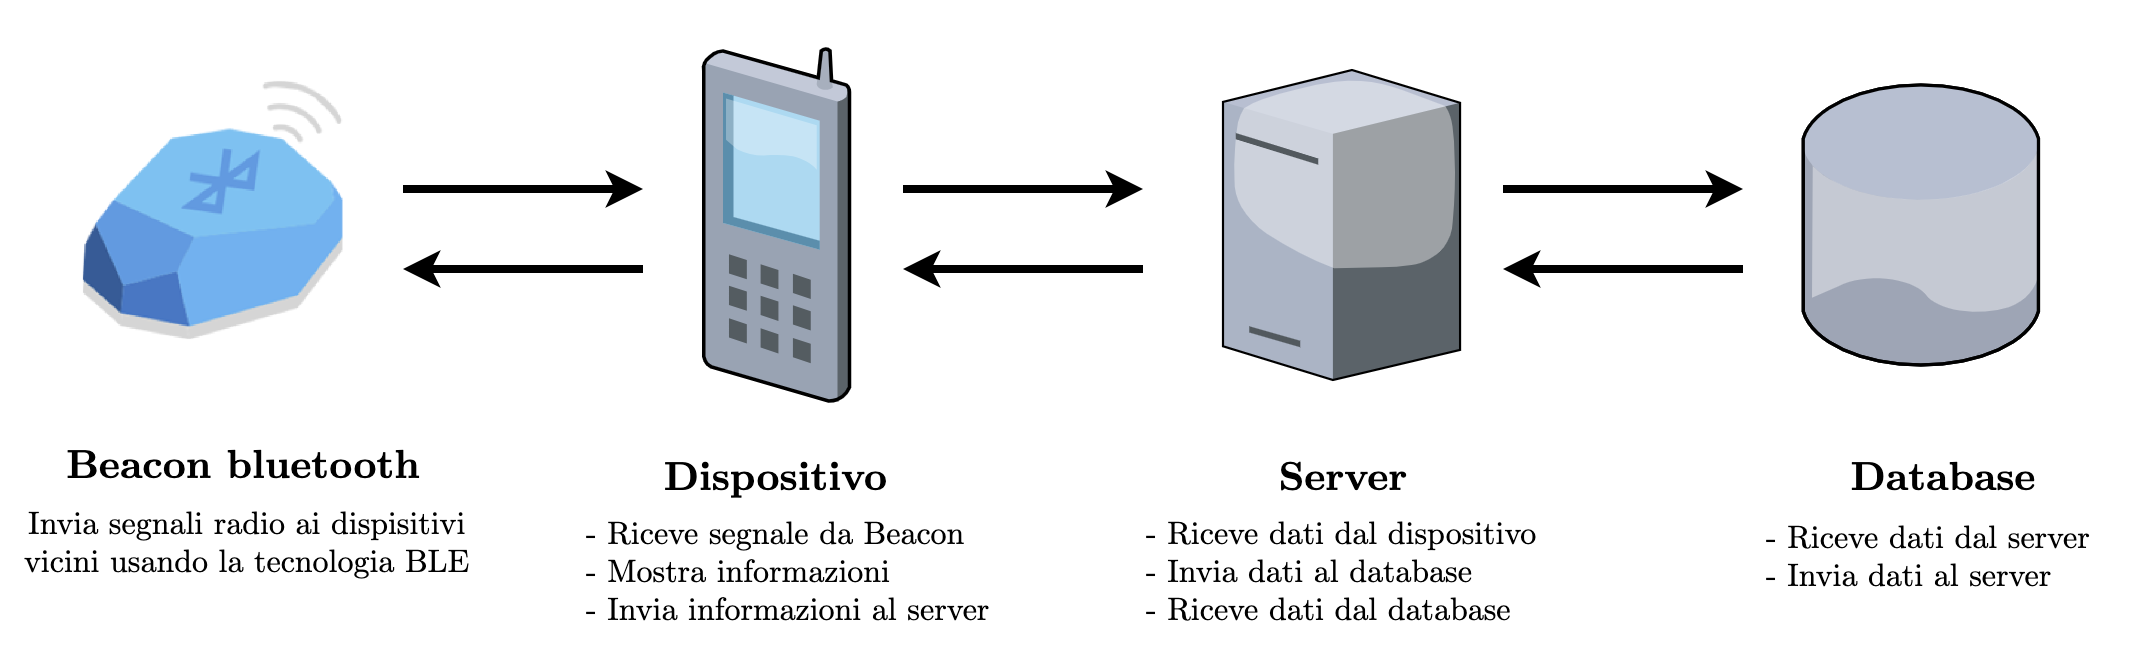
\includegraphics[width=15cm]{diagrams/diagramma_comunicazione.png}
    \caption{Architettura della comunicazione}
    \label{fig:architettura_comunicazione}
\end{figure}
\end{center}

\subsubsection{Utilizzare un beacon bluetooth}
Per realizzare un beacon Bluetooth vi sono farie opzioni:
\begin{enumerate}
    \item Acquistare un dispositivo già programmato con alimentazione propria ad un costo di circa 5/10 euro.
    \item Utilizzare un modulo Bluetooth BLE (ad esempio l'HM-10) e alimentarlo via USB
    \item Traformare il proprio telefono cellulare in un trasmettitore BLE con una semplice applicazione
\end{enumerate}

A seguito della natura dimostrativa di questo progetto è stata scelta la terza opzione.

\subsection{Internet of Things} Tutta questa interconnettività forma quello che viene chiamato \textbf{Internet of Things}, un termine che descrive l'estensione della connessione Internet alle più svariate tipologie di oggetti, in questo caso i beacon bluetooth. I dati rilevati grazie ad appositi sensori possono essere scambiati e comunicati tramite Internet e gli oggetti possono essere monitorati e gestiti da remoto.

% \subsubsection{HM-10}
% L'\textbf{HM10} è un modulo seriale BLE (Bluetooth-Low-Energy) destinato all'uso per applicazioni a basso consumo. È dotato di una interfaccia seriale/UART che rende il dispositivo in grado di interfacciarsi con diversi microcontrollori (vengono inviati comandi AT), tra cui appunto l'Arduino Uno. L'HM10 è un dispositivo economico e semplice da usare per creare connessioni semplici e usarlo come beacon Bluetooth.

% \begin{center}
% \begin{figure}[htp]
%     \centering
%     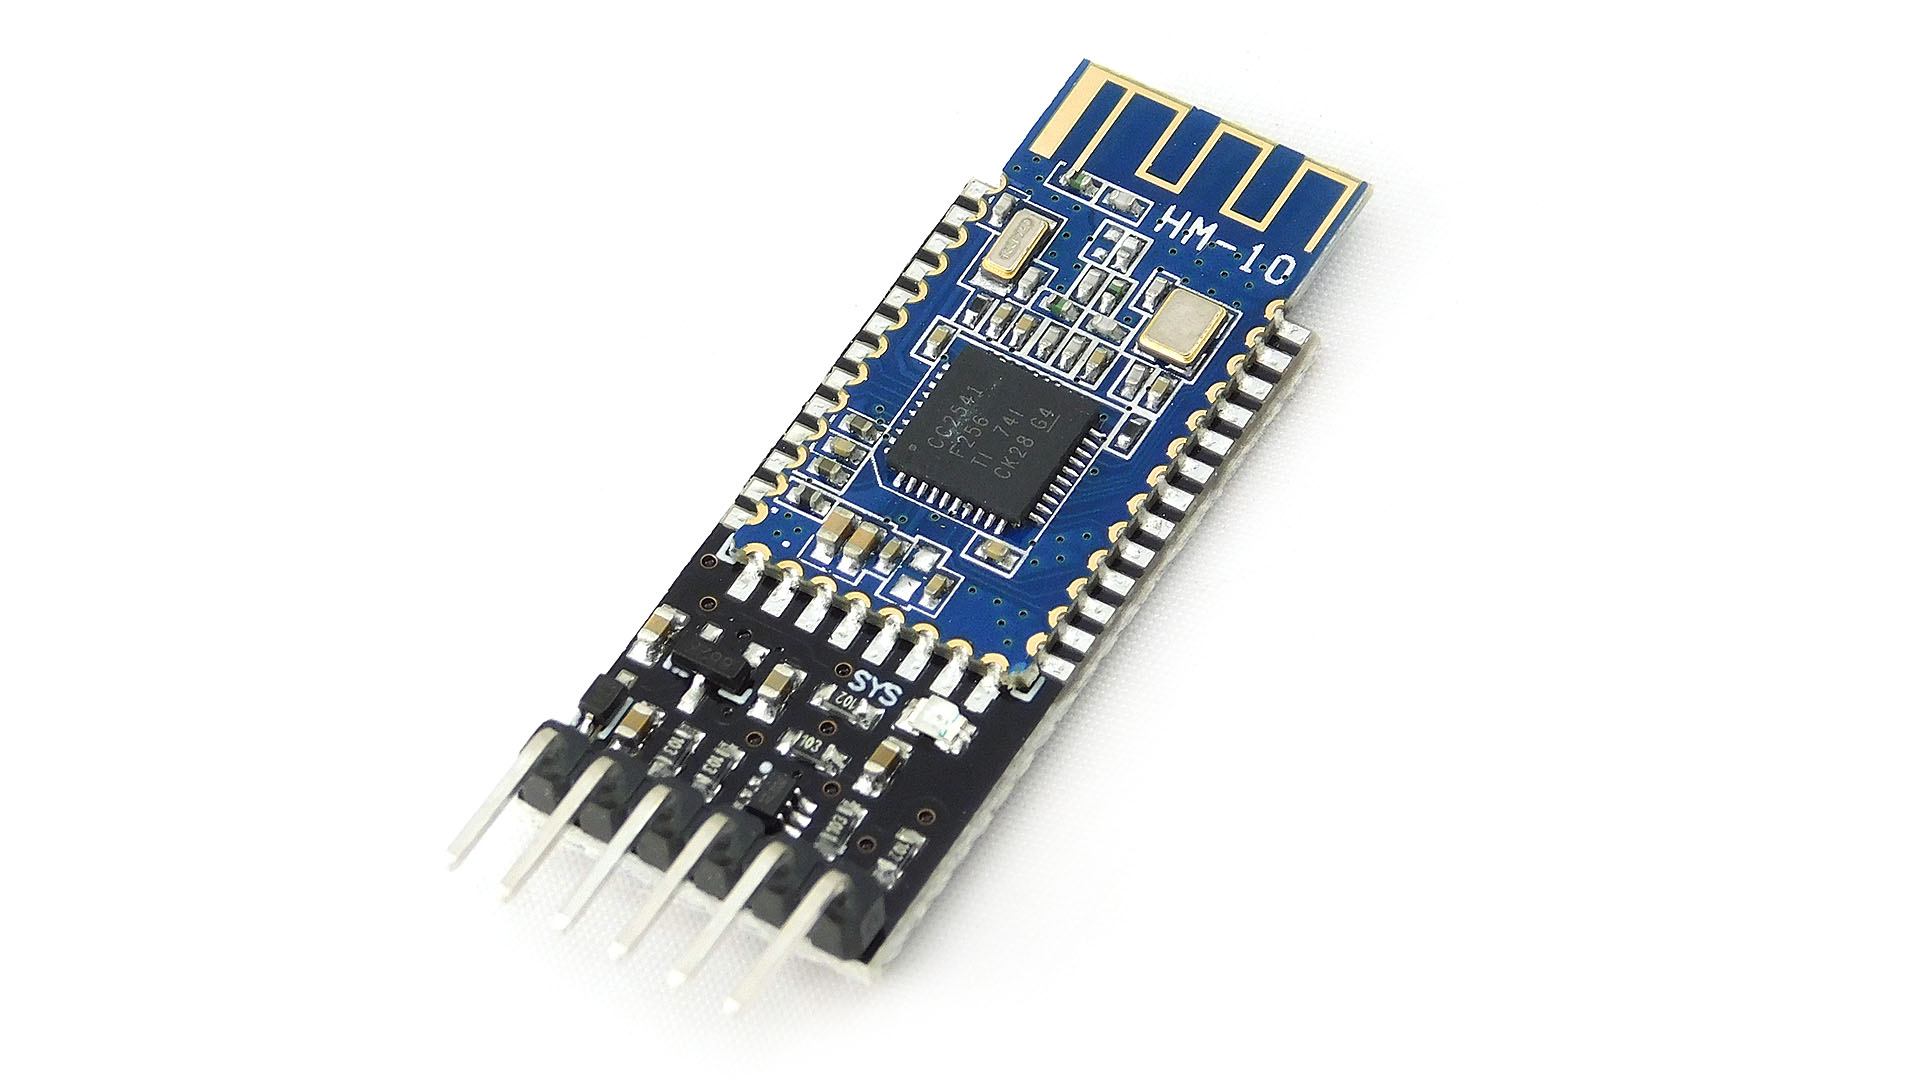
\includegraphics[width=8cm]{images/hm-10.jpeg}
%     \caption{Modulo HM-10}
%     \label{fig:hm_10}
% \end{figure}
% \end{center}

